% DRAFT: EGL research paper, IEEE conference format.
% Build:  pdflatex egl_paper && bibtex egl_paper && pdflatex egl_paper && pdflatex egl_paper
% Items in red (\TODO) are open before submission.
\documentclass[conference]{IEEEtran}
\IEEEoverridecommandlockouts
\usepackage{cite}
\usepackage{amsmath,amssymb}
\usepackage{graphicx}
\usepackage{booktabs}
\usepackage{xcolor}
\usepackage{algorithm}
\usepackage{algpseudocode}
\usepackage{tikz}
\usetikzlibrary{positioning,arrows.meta}
\usepackage[hidelinks]{hyperref}
\graphicspath{{figures/}}

\newcommand{\TODO}[1]{\textcolor{red}{[TODO: #1]}}
\newcommand{\x}{\ensuremath{\times}}

\begin{document}

\title{Don't Learn From Strangers: Frog-Boiling Poisoning of Adaptive SDN DDoS Detectors and an Evidence-Gated Defense}

\author{\IEEEauthorblockN{Anirudh Nambiar}
\IEEEauthorblockA{\textit{Dept.\ of Computer Science and Engineering}\\
\textit{National Institute of Technology Calicut}\\
Kozhikode, India\\
\TODO{email}}
\and
\IEEEauthorblockN{Arun Raj Kumar P}
\IEEEauthorblockA{\textit{Dept.\ of Computer Science and Engineering}\\
\textit{National Institute of Technology Calicut}\\
Kozhikode, India\\
\TODO{email}}
}

\maketitle

\begin{abstract}
Adaptive detectors are increasingly used to protect Software-Defined Networks (SDN) from DDoS attacks, because a fixed baseline raises false alarms whenever legitimate traffic grows. We show that this adaptivity is itself an attack surface. A frog-boiling attacker who raises a SYN flood slowly is learned as normal: in a Mininet/Ryu testbed, an EWMA detector that caught an abrupt $10\times$ flood in about one second missed the same flood in 9 of 11 runs when it ramped at 0.5--2\%/s, and an online machine learning detector (Half-Space Trees) was poisoned in the same way. We derive the condition under which such a ramp sustains itself. We then propose Evidence-Gated Learning (EGL), a detector-agnostic wrapper that lets a detector update its model only while the protected server completes the connections it is asked to open. EGL measures the ratio of server FINs to client SYNs with switch flow counters, with no Packet-In messages, and the evidence cannot be produced by off-path spoofed traffic. With EGL, EWMA detected every slow ramp (11/11 runs, at $2.7$--$2.9\times$ the normal rate, matching our analytical prediction of $2.9\times$) without additional false alarms on a $5\times$ legitimate flash crowd. The same evidence identifies verified clients: a mitigation that meters unverified SYNs and lets verified clients bypass the meter reduced failed or delayed user requests during a $10\times$ flood from 34.5\% to 0.4\%, whereas a plain SYN meter raised them to 87.7\%.
\end{abstract}

\begin{IEEEkeywords}
Software-defined networking, DDoS, poisoning attacks, online anomaly detection, SYN flood, OpenFlow
\end{IEEEkeywords}

% =====================================================================
\section{Introduction}
% =====================================================================
Software-Defined Networking (SDN) gives a logically centralized controller a global view of the network and the ability to program every switch \cite{mckeown2008openflow,kreutz2015sdn}. This makes the controller a natural place to detect and mitigate Distributed Denial of Service (DDoS) attacks, and a large body of work does so with statistical thresholds, entropy measures and machine learning \cite{yan2016sdnddos,braga2010som,mousavi2015entropy}.

Real traffic is not stationary. It follows daily cycles and sudden legitimate surges (flash crowds), so a detector with a fixed baseline raises false alarms whenever legitimate load grows. Recent SDN detectors therefore \emph{adapt}: they keep updating their notion of normal traffic, typically only from windows they classify as normal \cite{zhang2026time}. Online machine learning detectors such as Half-Space Trees adapt in the same way \cite{tan2011hst}.

Adaptation creates an opening. An attacker who increases a flood slowly keeps every observation within the detector's tolerance. The detector learns each step, its baseline follows the attack, and the flood can reach many times the normal rate without an alarm. This \emph{frog-boiling} or poisoning attack is known for backbone anomaly detectors \cite{rubinstein2009antidote} and network coordinate systems \cite{chantin2009frog}. To our knowledge it has not been studied for SDN DDoS detectors, and recent adaptive SDN detectors explicitly leave adaptive attackers out of scope \cite{zhang2026time}.

The root of the problem is that an adaptive detector decides \emph{what to learn} using its own judgement of normality, which is exactly what a slow attack is built to pass. We argue that this decision should instead rest on independent evidence that the traffic is legitimate. For TCP services such evidence is cheap: legitimate clients complete their connections, so the protected server closes them, while spoofed SYNs never complete \cite{wang2002syn}.

This paper makes the following contributions:
\begin{itemize}
\item We demonstrate frog-boiling attacks against adaptive SDN DDoS detectors, both a statistical detector (EWMA) and an online machine learning detector (Half-Space Trees), and derive when a ramp is self-sustaining against EWMA (Section~\ref{sec:attack}).
\item We propose Evidence-Gated Learning (EGL), a detector-agnostic wrapper that permits learning only while the server completes connections. Its evidence is collected with flow counters on the server's switch port, so it needs no Packet-In messages and cannot be produced by off-path spoofed traffic (Section~\ref{sec:egl}).
\item We use the same evidence for selective mitigation: an OpenFlow meter on unverified SYNs with per-client bypass rules for verified clients.
\item We evaluate EGL in Mininet with Ryu and Open vSwitch over 69 live runs, with offline replay for parameter studies, and report its limits, notably attackers that complete real connections (Sections~\ref{sec:eval}--\ref{sec:discussion}).
\end{itemize}

% =====================================================================
\section{Background and Related Work}\label{sec:related}
% =====================================================================
\textbf{DDoS detection in SDN.} Surveys classify SDN DDoS defences into statistical, entropy-based and machine-learning approaches \cite{yan2016sdnddos}. Early work used self-organizing maps over flow features collected by the controller \cite{braga2010som} and the entropy of destination addresses \cite{mousavi2015entropy}. Fixed thresholds false-alarm on flash crowds; recent work therefore adapts the threshold. Zhang et al.\ combine temporal and spatial entropy with an EWMA-style dynamic threshold that is updated from windows classified as normal, evaluated in Mininet with Ryu \cite{zhang2026time}. Online anomaly detectors such as Half-Space Trees learn from a stream without labels and follow drift by periodically renewing their reference model \cite{tan2011hst}. Both kinds of detectors decide what to learn from their own verdicts, which is the property we attack.

\textbf{SYN floods in SDN.} AVANT-GUARD adds connection migration to switches, so that only clients that complete the TCP handshake reach the controller and the server \cite{shin2013avantguard}. FloodGuard protects the controller from Packet-In floods with proactive rules and a packet migration cache \cite{wang2015floodguard}. Both require extensions to the switch or controller data path. EGL uses only OpenFlow 1.3 tables, meters and counters, and it complements detectors rather than replacing them.

\textbf{Protocol evidence.} Wang et al.\ observed that SYN and FIN (or RST) packets come in pairs in normal TCP traffic, and detected SYN floods with a CUSUM test on their difference at leaf routers \cite{wang2002syn}. We use the same evidence for a different purpose: not as a detector, but to decide when an adaptive detector may learn.

\textbf{Poisoning of adaptive detectors.} Rubinstein et al.\ poisoned PCA-based backbone anomaly detectors by injecting small amounts of traffic over time, including a ``boiling frog'' strategy, and proposed robust PCA (ANTIDOTE) to limit the damage \cite{rubinstein2009antidote}. Chan-Tin et al.\ showed that frog-boiling defeats anomaly detection in network coordinate systems \cite{chantin2009frog}. Robust statistics bound how much each poisoned point can move the model, but a sufficiently slow attacker still succeeds. EGL instead stops learning when the evidence disappears.

% =====================================================================
\section{Threat Model}\label{sec:threat}
% =====================================================================
The defender is an SDN controller protecting a TCP service (here a web server) attached to an OpenFlow switch. The attacker controls hosts on one or more switches, may spoof source addresses, and chooses the SYN rate in every second. The attacker knows the detector's algorithm and parameters but not its current state, and can estimate the legitimate load. The goal is to raise the SYN rate to a target amplification $F$ (e.g., $10\times$ the legitimate rate) without triggering an alarm, or to make mitigation harm legitimate users. The attacker cannot compromise the controller, the switches or the server, and cannot inject packets that enter the switch on the server's port. Attackers that complete real TCP connections from real addresses (application-layer floods) are outside this model; we measure them as a limitation in Section~\ref{sec:eval}.

% =====================================================================
\section{Frog-Boiling Adaptive Detectors}\label{sec:attack}
% =====================================================================
Consider an EWMA detector on the SYN rate $x_n$ with learning weight $\beta$ and alarm width $\kappa$:
\begin{align}
\mu_{n+1} &= \mu_n + \beta (x_n - \mu_n),\\
\sigma^2_{n+1} &= (1-\beta)\,\sigma^2_n + \beta (x_n-\mu_n)^2,
\end{align}
raising an alarm when $x_n > \mu_n + \kappa\sigma_n$ and updating only when it does not alarm. Let the attacker grow the SYN rate geometrically, $x_n = x_0 (1+r)^n$. In steady state the baseline trails the attack by a constant factor:
\begin{equation}
\frac{x_n}{\mu_n} = 1 + g, \qquad g = \frac{r}{\beta}. \label{eq:lag}
\end{equation}
The deviation $x_n - \mu_n = g\mu_n$ also enters the variance, whose steady state is $\sigma_n^2 = \mu_n^2\, \beta g^2 / \big((1+r)^2 - 1 + \beta\big)$. The alarm condition $g\mu_n > \kappa\sigma_n$ therefore never holds when
\begin{equation}
\kappa^2 \beta \ge (1+r)^2 - 1 + \beta \;\;\Longleftrightarrow\;\; r \lesssim \tfrac{1}{2}\beta(\kappa^2 - 1). \label{eq:sustain}
\end{equation}
For $\beta = 0.1$ and $\kappa = 3$ this admits any ramp slower than about 40\% per second. Such a ramp is \emph{self-sustaining}: it inflates the very variance that would expose it. Reaching amplification $F$ takes
\begin{equation}
n = \frac{\ln F}{\ln(1+r)} = \frac{\ln F}{\ln(1+\beta g)} \ \text{seconds}, \label{eq:time}
\end{equation}
for example 116~s for $F = 10$ at $r = 2\%$/s ($g = 0.2$). Only noise spikes larger than the alarm width can reveal the attack, which is why the plain EWMA detector in our experiments caught slow ramps only occasionally, and late. Fig.~\ref{fig:frog} shows the effect live: the same $10\times$ flood raises its first alarm after 1.2~s (31 alarms in total) when abrupt, and none when it ramps at 2\%/s to $10.3\times$.

\begin{figure}[t]
\centering
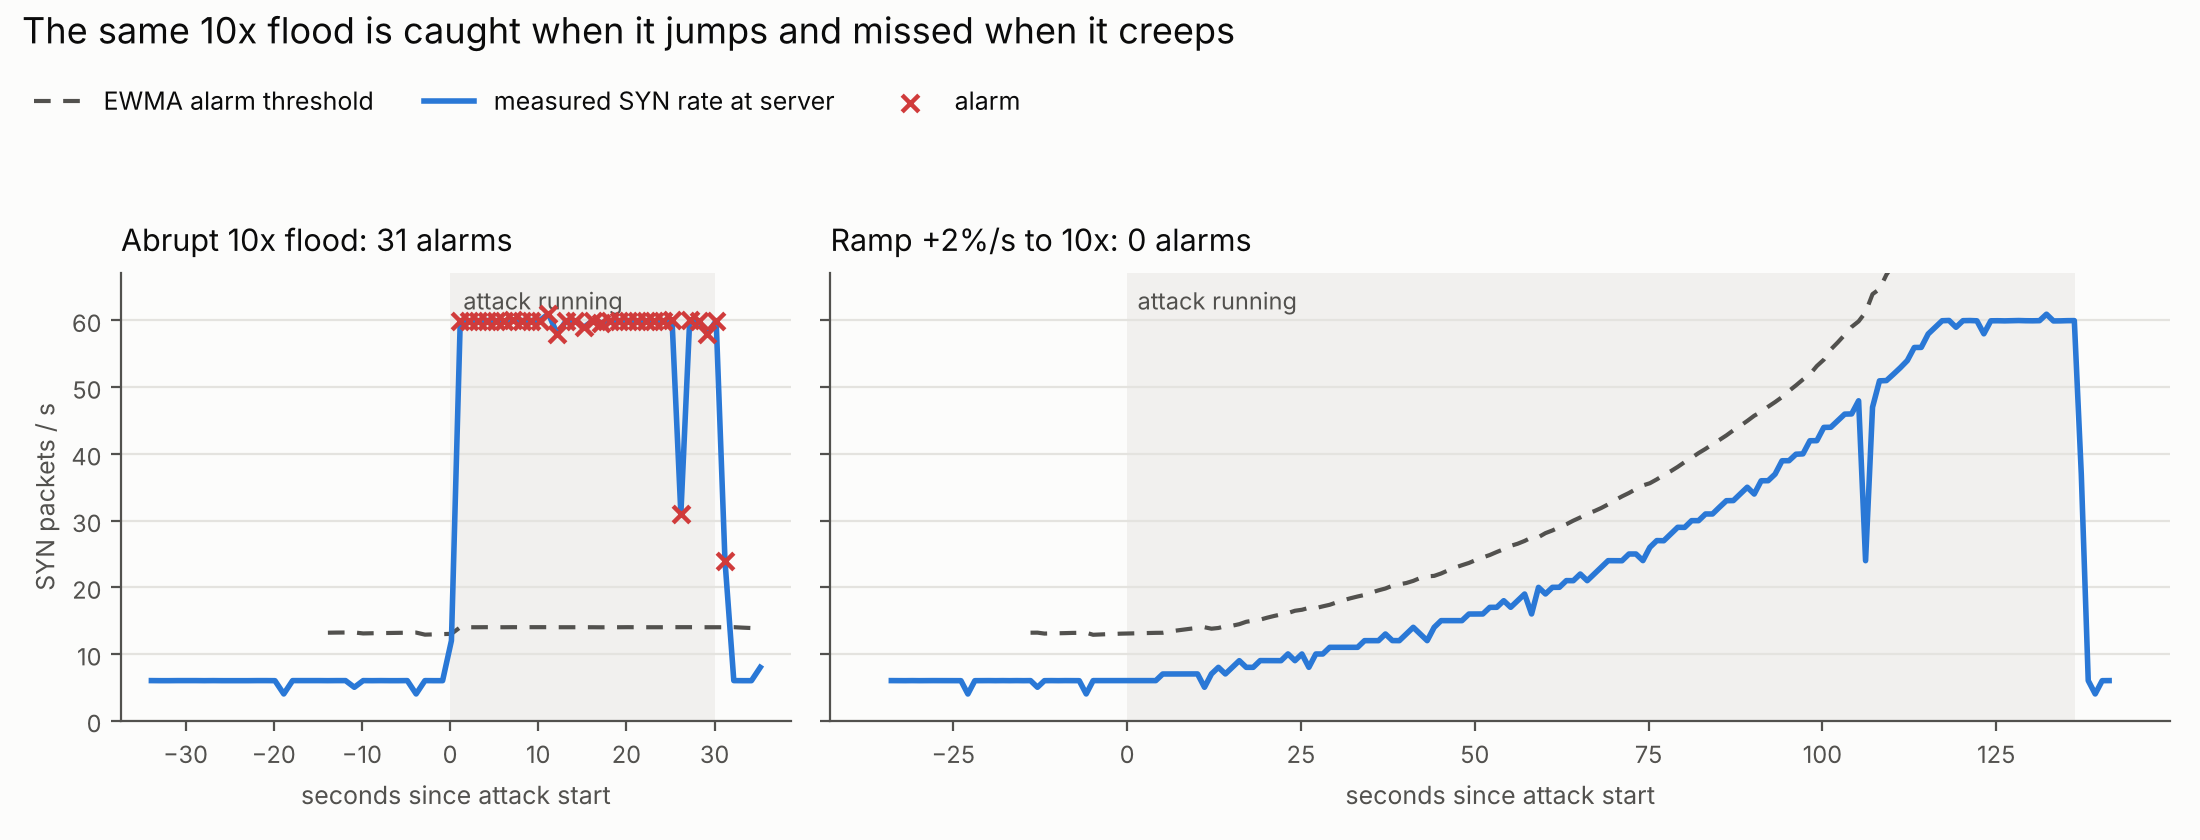
\includegraphics[width=\columnwidth]{step2_ramp_vs_abrupt.png}
\caption{The same $10\times$ SYN flood against an EWMA detector: abrupt (left) it is caught after 1.2~s; ramped at 2\%/s (right) it reaches $10.3\times$ with zero alarms.}
\label{fig:frog}
\end{figure}

Any detector that adapts from its own verdicts has the same weakness. Half-Space Trees renew their reference model every window from recent points, so a ramp that is slow relative to the window becomes the new reference. Section~\ref{sec:eval} confirms this experimentally.

% =====================================================================
\section{Evidence-Gated Learning}\label{sec:egl}
% =====================================================================
\begin{figure*}[t]
\centering
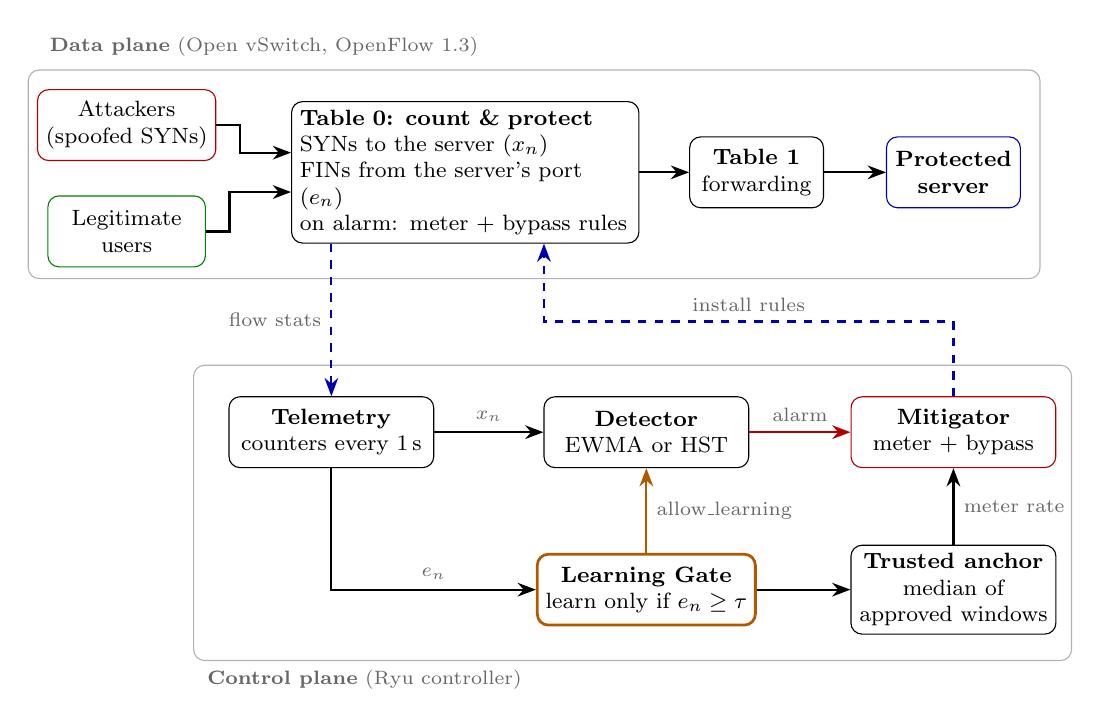
\begin{tikzpicture}[x=1cm,y=1cm,>=Stealth,
  b/.style={draw,rounded corners,align=center,font=\footnotesize,inner sep=3pt,minimum height=9mm},
  st/.style={b,minimum width=26mm},
  arr/.style={->,thick},
  ctl/.style={->,thick,dashed,blue!70!black},
  lbl/.style={font=\scriptsize,text=black!60,align=center}]
\node[b,draw=red!70!black,minimum width=20mm] (atk) at (0,0.6) {Attackers\\(spoofed SYNs)};
\node[b,draw=green!50!black,minimum width=20mm] (usr) at (0,-0.75) {Legitimate\\users};
\node[b,align=left,text width=42mm] (t0) at (4.3,0) {\textbf{Table 0: count \& protect}\\SYNs to the server ($x_n$)\\FINs from the server's port ($e_n$)\\on alarm: meter + bypass rules};
\node[b,minimum width=17mm] (t1) at (8.0,0) {\textbf{Table 1}\\forwarding};
\node[b,draw=blue!70!black,minimum width=17mm] (srv) at (10.5,0) {\textbf{Protected}\\\textbf{server}};
\draw[arr] (atk.east) -- ++(0.3,0) |- ([yshift=2.5mm]t0.west);
\draw[arr] (usr.east) -- ++(0.3,0) |- ([yshift=-2.5mm]t0.west);
\draw[arr] (t0) -- (t1); \draw[arr] (t1) -- (srv);
\node[lbl,anchor=south west] at (-1.1,1.35) {\textbf{Data plane} (Open vSwitch, OpenFlow 1.3)};
\draw[black!30,rounded corners] (-1.25,-1.35) rectangle (11.6,1.3);
\node[st] (tel) at (2.6,-3.3) {\textbf{Telemetry}\\counters every 1\,s};
\node[st] (det) at (6.6,-3.3) {\textbf{Detector}\\EWMA or HST};
\node[st,draw=red!70!black] (mit) at (10.5,-3.3) {\textbf{Mitigator}\\meter + bypass};
\node[st,draw=orange!70!black,line width=1pt] (gate) at (6.6,-5.3) {\textbf{Learning Gate}\\learn only if $e_n \ge \tau$};
\node[st] (base) at (10.5,-5.3) {\textbf{Trusted anchor}\\median of\\approved windows};
\draw[arr] (tel) -- node[lbl,above]{$x_n$} (det);
\draw[arr,red!70!black] (det) -- node[lbl,above]{alarm} (mit);
\draw[arr] (tel.south) |- node[lbl,above,pos=0.75]{$e_n$} (gate.west);
\draw[arr,orange!70!black] (gate) -- node[lbl,right]{allow\_learning} (det);
\draw[arr] (gate) -- (base); \draw[arr] (base) -- node[lbl,right]{meter rate} (mit);
\node[lbl,anchor=north west] at (0.9,-6.2) {\textbf{Control plane} (Ryu controller)};
\draw[black!30,rounded corners] (0.85,-6.2) rectangle (12.0,-2.45);
\draw[ctl] (t0.south -| tel) -- node[lbl,left]{flow stats} (tel.north);
\draw[ctl] (mit.north) -- ++(0,0.95) -| node[lbl,above,pos=0.25]{install rules} ([xshift=10mm]t0.south);
\end{tikzpicture}
\caption{EGL architecture. Flow counters in table~0 provide the SYN rate $x_n$ and the completion ratio $e_n$; the Learning Gate decides whether the detector may learn; alarms trigger selective mitigation sized from the gate's trusted anchor.}
\label{fig:arch}
\end{figure*}

\subsection{Completion evidence}
EGL rests on one observation: a legitimate client that opens a TCP connection eventually receives a FIN from the server, whereas a spoofed SYN never completes. We define the completion ratio over a window $W$ (5~s in our implementation) as
\begin{equation}
e_n = \frac{\sum_{W} \text{FINs sent by the server}}{\sum_{W} \text{SYNs sent to the server}} . \label{eq:completion}
\end{equation}
For legitimate traffic $e_n \approx 1$, including during a flash crowd. If an attack adds spoofed SYNs so that the total is $m$ times the legitimate rate, then $e_n \approx 1/m$. The ratio is undefined when fewer than 3 SYNs were seen in the window.

The evidence is collected entirely in the switch. Table~0 of the server's switch holds counting rules that match on TCP flags (an ONF extension to OpenFlow 1.3, standard in OpenFlow 1.5, supported by Open vSwitch): client SYNs to the server (SYN set, ACK clear) and server FINs (FIN set). The FIN rule also matches \texttt{in\_port} = the server's port, so off-path hosts cannot add to it even with spoofed source addresses. Each rule forwards to table~1, which performs normal forwarding. The controller polls the flow and port statistics once per second. No Packet-In messages are used for telemetry, so the controller's monitoring cost is independent of the attack rate.

\subsection{The Learning Gate}
The gate sits between telemetry and any online detector. In each second it opens if $e_n \ge \tau$ or if $e_n$ is undefined (almost no traffic), and closes otherwise. The detector may update its model only if it raised no alarm \emph{and} the gate is open (Algorithm~\ref{alg:egl}). The gate never raises alarms itself; it only decides what the detector learns, so it can wrap any detector that learns online. The detectors never see $e_n$.

With an attack at $m$ times the legitimate rate, the gate closes when $1/m < \tau$, i.e.\ at
\begin{equation}
m^{*} = 1/\tau \qquad (m^{*} \approx 1.43 \text{ for } \tau = 0.7). \label{eq:mstar}
\end{equation}
From then on the EWMA baseline is frozen near $m^{*} r_0$, where $r_0$ is the legitimate SYN rate. With $\sigma$ at its Poisson floor $\sqrt{\mu}$, the attack is detected at an amplification of roughly
\begin{equation}
A \approx m^{*} + \kappa \frac{\sqrt{m^{*} r_0}}{r_0} , \label{eq:pred}
\end{equation}
which for $r_0 \approx 6$~SYN/s, $\tau = 0.7$ and $\kappa = 3$ gives $A \approx 2.9$. Notably, $A$ does not depend on the ramp speed $r$.

\begin{algorithm}[t]
\caption{Evidence-gated detection, executed every second}\label{alg:egl}
\begin{algorithmic}[1]
\Require counters $c_n$, detector $D$ with model $\theta$, threshold $\tau$
\State $x_n \gets$ SYN rate from $c_n - c_{n-1}$
\State $e_n \gets$ completion ratio over the last $W$ seconds \Comment{Eq.~\eqref{eq:completion}}
\State $a_n \gets D.\mathrm{score}(x_n; \theta)$ \Comment{no alarms during warm-up}
\State $open \gets (e_n \text{ undefined}) \lor (e_n \ge \tau)$
\If{$open$ \textbf{and} $e_n$ defined} add $x_n$ to the trusted anchor \EndIf
\If{$a_n = 0$ \textbf{and} $open$} $\theta \gets D.\mathrm{update}(\theta, x_n)$ \EndIf
\If{$a_n = 1$} raise alarm to the mitigator \EndIf
\end{algorithmic}
\end{algorithm}

\textbf{Trusted anchor.} The gate keeps the median (with MAD) of the SYN rates of the windows it approved. This anchor estimates the legitimate rate even after the detector's model has stopped learning, and the mitigator uses it to size its meter.

\textbf{Gated warm-up.} A detector must first learn an initial model. In our first version every warm-up second was learned regardless of the gate, so a flood that began during warm-up became part of the initial model and was never detected. In the final design a warm-up second counts only if the gate accepts it. If the gate keeps rejecting, warm-up ends after three times its normal length using the accepted seconds collected so far (at least five). Half-Space Trees also calibrate their alarm threshold only on accepted seconds.

\textbf{Optional drift budget.} To study attackers that complete connections, the gate can additionally refuse to learn windows that would move the anchor faster than $\delta$ per second. This is off by default, for reasons shown in Section~\ref{sec:eval}.

\subsection{Selective mitigation with verified clients}
A plain SYN meter is a poor response to a spoofed flood: during a $10\times$ flood about nine in ten SYNs are spoofed, so the meter mostly drops legitimate users' SYNs. EGL reuses its evidence. The server-FIN rule also copies FINs to the controller; the destination of each FIN is a client that has just completed a connection, and is recorded as \emph{verified}. A spoofed address can never become verified. When the protected detector raises an alarm, the mitigator (i) installs an OpenFlow meter limiting SYNs to the server to $\max(1.5\,\hat{r}, 5)$ per second, where $\hat{r}$ is the trusted anchor, and (ii) installs, for every client verified in the last 10 minutes, a higher-priority rule that lets its SYNs skip the meter. Bypass rules still count SYNs, so telemetry is unaffected. New clients verified during the attack receive bypass rules as they appear, and all rules are removed 10~s after the alarm clears.

% =====================================================================
\section{Implementation and Testbed}\label{sec:impl}
% =====================================================================
EGL is implemented in Python as three Ryu 4.34 \cite{ryu} applications using OpenFlow 1.3 \cite{onf2012of13}: a controller application (pipeline, polling, completion ratio), a detector application that runs all detectors with and without the gate on the same telemetry, and a mitigator. The network is emulated in Mininet \cite{lantz2010mininet} with Open vSwitch \cite{pfaff2015ovs}.

\textbf{Detectors.} \emph{Static}: mean and standard deviation from warm-up, alarm at $z > 3$, no further learning. \emph{EWMA}: $\beta = 0.1$, $\kappa = 3$, $\sigma \ge \sqrt{\mu}$, learning only from non-alarm windows. \emph{Half-Space Trees} (HST) \cite{tan2011hst}: 25 trees of depth 10 over $\log$ SYN rate and $\log$ packets to the server, window 20~s, alarm threshold $0.5\times$ the minimum calibration score. EWMA+gate and HST+gate wrap the same detectors with the Learning Gate ($\tau = 0.7$, $W = 5$~s).

\textbf{Topology and traffic.} Three switches (two access switches connected to a core switch) and twelve hosts. The server runs a threaded HTTP server with a backlog of 511 and SYN cookies disabled; its default gateway is a sink host, so SYN-ACKs to spoofed addresses leave the network. Three legitimate users each request a page every 0.5~s (about 6~SYN/s in total); in mitigation runs each user host draws its source address from a pool of 20, and the server treats every visitor as new. A raw-socket generator sends spoofed SYNs on an exact per-second schedule; the switch counted 98--99\% of planned packets. In the main evaluation the attack is sent from one host; in the distributed experiments it is split across three hosts, one on each switch.

\textbf{Scenarios.} (i) \emph{Abrupt}: a step to $10\times$ (about 60~SYN/s). (ii) \emph{Ramp}: geometric growth at $r \in \{0.5, 1, 2\}\%$/s to $10\times$. (iii) \emph{Flash crowd}: no attack; legitimate users grow from 3 to 15 within 60~s; any alarm is false. (iv) \emph{Completing bots}: bots with real addresses that complete HTTP requests, ramping at 2\%/s. (v) \emph{Early}: an abrupt flood starting 10~s after the users, inside warm-up. Every run begins with 60~s of legitimate traffic.

% =====================================================================
\section{Evaluation}\label{sec:eval}
% =====================================================================
\textbf{Setup and metrics.} The main evaluation (57 runs) ran on a laptop (Ubuntu on WSL2) with the Open vSwitch kernel datapath, with the attack sent from a single host. Twelve further runs (the early-attack and distributed-attack stages) ran in a cloud container with the user-space datapath. We report detection rate, time to first alarm, \emph{amplification at first alarm} (attack rate over the legitimate rate), runs with false alarms in the flash crowd, the share of user requests that failed or were delayed (needed a SYN retransmission, i.e.\ at least about 1~s extra), and the peak number of half-open connections at the server. Values are mean $\pm$ 95\% confidence interval over repeated runs. Parameter studies replay the recorded telemetry offline, so every setting sees identical traffic.

\subsection{Are adaptive detectors vulnerable?}
Table~\ref{tab:detection} shows that every detector catches the abrupt flood in about one second. On the slow ramp, EWMA raised an alarm in only 1 of 5 runs, at $10.2\times$; the single HST detection was an alarm on a brief traffic dip, not on the attack. Across all three ramp speeds (Table~\ref{tab:growth}), plain EWMA caught the ramp in 2 of 11 runs, each time above $10\times$. Static detects ramps at about $2.2\times$, but raises a false alarm in every flash crowd. HST is both poisoned by the slowest ramp and alarms on every crowd.

\begin{table}[t]
\centering
\caption{Detection (5 runs per scenario; ramp at 0.5\%/s)}
\label{tab:detection}
\setlength{\tabcolsep}{3.5pt}
\begin{tabular}{lccc}
\toprule
Detector & Abrupt $10\times$ & Ramp: detected (ampl.) & Crowd FA \\
\midrule
Static & 5/5 (1.1 s) & 5/5 ($2.17 \pm 0.11\times$) & 5/5 \\
EWMA & 5/5 (1.1 s) & 1/5 ($10.21\times$) & 1/5 \\
HST & 5/5 (1.1 s) & 1/5 ($0.52\times$)$^{\dagger}$ & 5/5 \\
\textbf{EWMA+gate} & \textbf{5/5 (1.1 s)} & \textbf{5/5 ($2.89 \pm 0.11\times$)} & \textbf{1/5} \\
HST+gate & 5/5 (1.1 s) & 5/5 ($1.93 \pm 1.02\times$) & 5/5 \\
\bottomrule
\multicolumn{4}{l}{\footnotesize $^{\dagger}$ An alarm on a brief traffic dip, not on the attack.}
\end{tabular}
\end{table}

\begin{table}[t]
\centering
\caption{Ramp speed: runs detected (amplification at alarm)}
\label{tab:growth}
\setlength{\tabcolsep}{3pt}
\begin{tabular}{lccc}
\toprule
Detector & 0.5\%/s (5) & 1\%/s (3) & 2\%/s (3) \\
\midrule
Static & 5/5 ($2.17\times$) & 3/3 ($2.25\times$) & 3/3 ($2.19\times$) \\
EWMA & 1/5 ($10.21\times$) & 1/3 ($15.23\times$) & 0/3 \\
HST & 1/5 & 2/3 ($3.27\times$) & 3/3 ($5.04\times$) \\
\textbf{EWMA+gate} & \textbf{5/5 ($2.89\times$)} & \textbf{3/3 ($2.83\times$)} & \textbf{3/3 ($2.72\times$)} \\
HST+gate & 5/5 ($1.93\times$) & 3/3 ($1.96\times$) & 3/3 ($2.54\times$) \\
\bottomrule
\end{tabular}
\end{table}

\subsection{Does EGL restore detection without false alarms?}
EWMA+gate detected the ramp in all 11 runs, at $2.72$--$2.89\times$ regardless of ramp speed, and remained quiet in 4 of 5 flash crowds. The one false alarm occurred in the same run with and without the gate, so it is EWMA's own and not caused by EGL. The gate closed at $1.43\times$, as predicted by Eq.~\eqref{eq:mstar}, and the measured detection point ($2.89 \pm 0.11\times$) matches the prediction of Eq.~\eqref{eq:pred} ($\approx 2.9\times$). The gate never closed in any of the 11 flash-crowd runs without a plain meter. Fig.~\ref{fig:detectors} shows one run of each scenario.

The gate controls learning, not alarming: HST+gate detects every ramp but still false-alarms on every crowd, because HST's alarm rule itself fires on rapid legitimate growth.

\begin{figure*}[t]
\centering
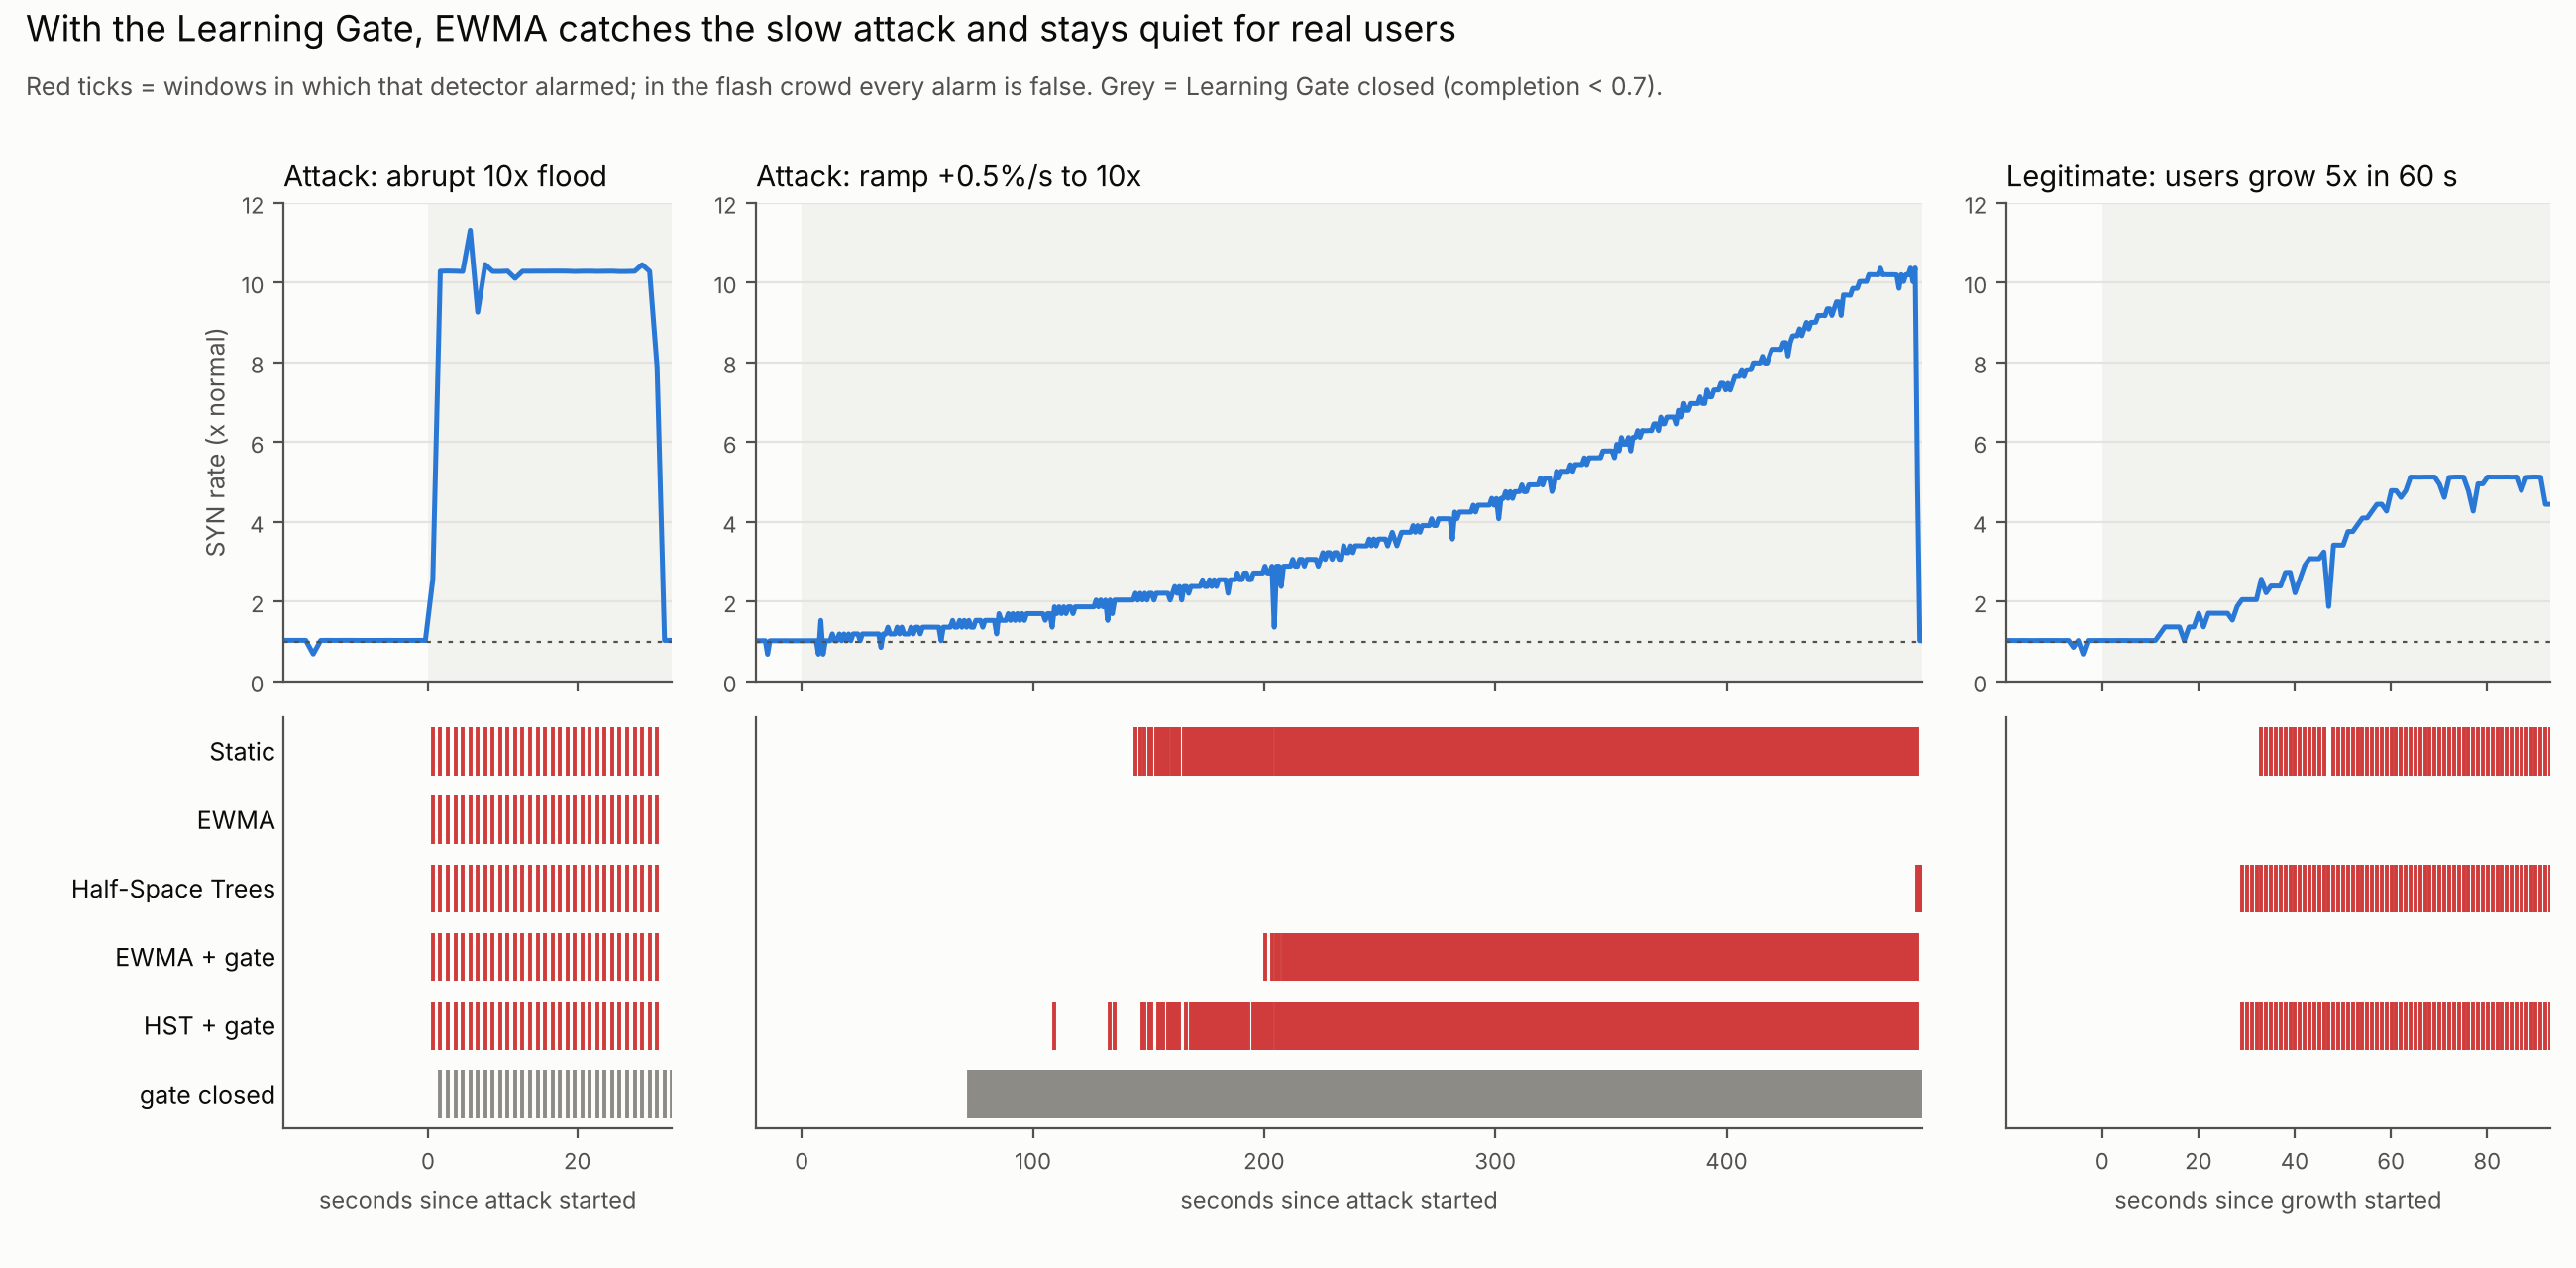
\includegraphics[width=0.9\textwidth]{step4_detectors.png}
\caption{One run each of the abrupt flood, slow ramp and flash crowd. Red marks are alarms; grey shading marks seconds in which the Learning Gate was closed.}
\label{fig:detectors}
\end{figure*}

\textbf{Choice of $\tau$.} Offline replay (Fig.~\ref{fig:tau}) shows that a higher $\tau$ freezes the model earlier and detects the ramp at a smaller amplification ($5.65\times$ at $\tau = 0.3$, $2.89\times$ at $0.7$, $2.34\times$ at $0.95$), consistent with Eq.~\eqref{eq:pred}. Crowd false alarms stay at 1/5 for every $\tau$, because legitimate crowds keep $e_n$ near 1. We use $\tau = 0.7$ to leave room for normal connection failures.

\begin{figure}[t]
\centering
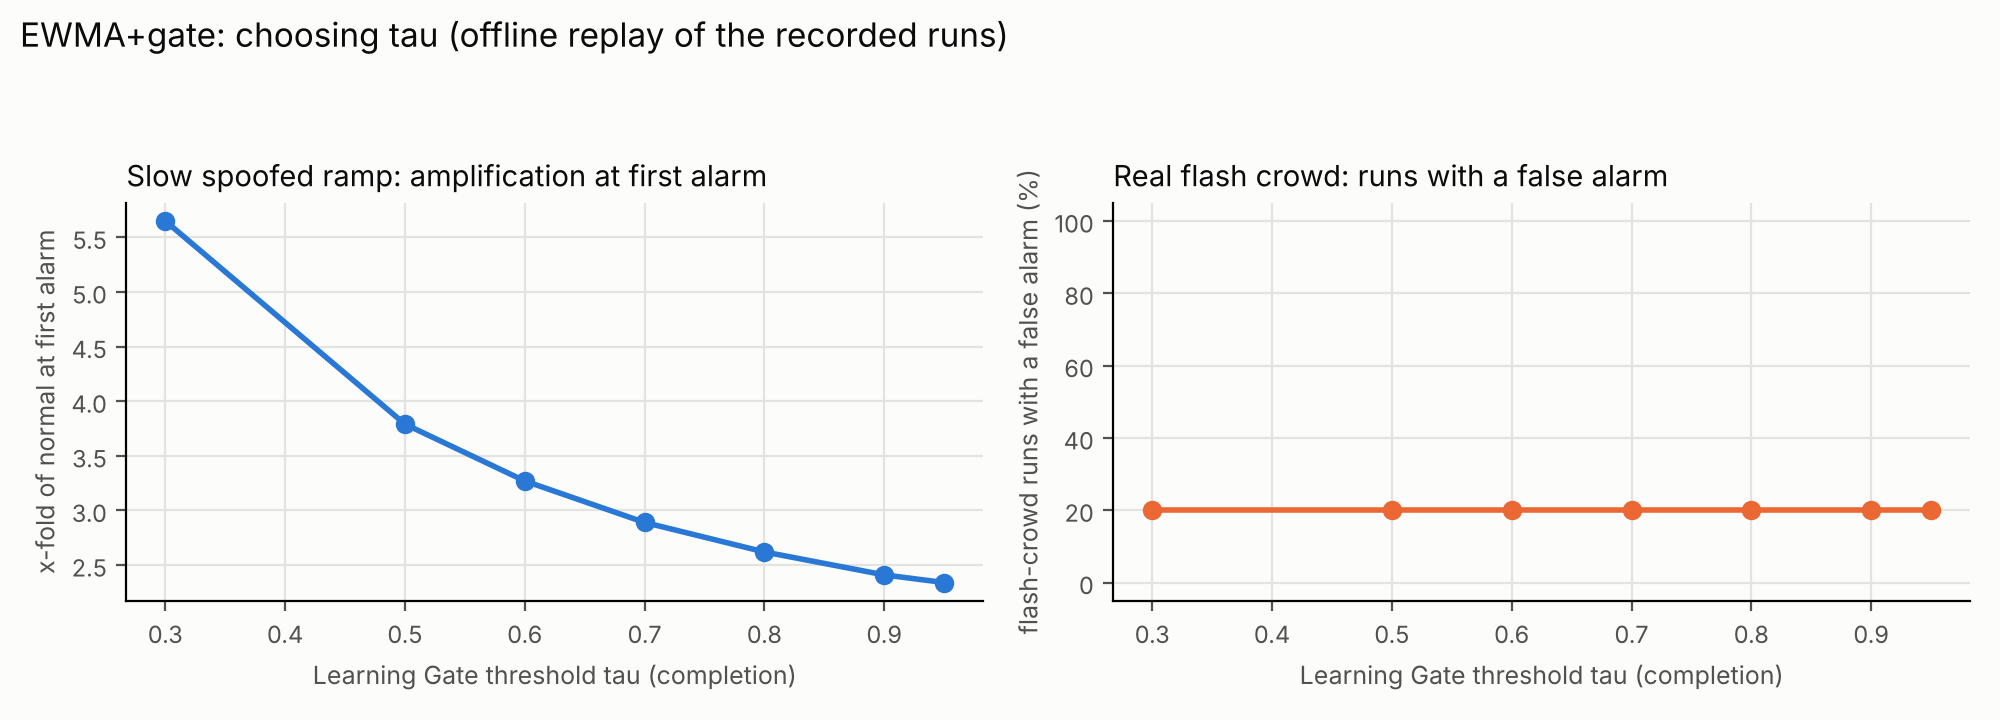
\includegraphics[width=\columnwidth]{fig_tau.png}
\caption{Effect of the gate threshold $\tau$ (offline replay, EWMA+gate).}
\label{fig:tau}
\end{figure}

\subsection{Robustness: early and distributed attacks}
Table~\ref{tab:robust} reports the attack that starts during warm-up. Without gated warm-up, all detectors, including the first version of EGL, learned the flood as part of their initial model (0/3). With gated warm-up, EWMA+gate and HST+gate detected it in all runs, 49~s after onset, when the extended warm-up ended. Replaying all 48 earlier gated runs with the final code produces identical results, so the change does not affect the other experiments. Splitting the attack across three hosts on all three switches gave results consistent with the single-host runs, since the detector observes aggregate traffic at the server.

\begin{table}[t]
\centering
\caption{Attack during warm-up (3 runs) and distributed attack}
\label{tab:robust}
\setlength{\tabcolsep}{3pt}
\begin{tabular}{lc}
\toprule
Case & Result \\
\midrule
Early flood: Static, EWMA, HST & 0/3 \\
Early flood: EWMA/HST+gate, ungated warm-up & 0/3 \\
\textbf{Early flood: EWMA/HST+gate, gated warm-up} & \textbf{3/3 (49 s)} \\
\midrule
3 hosts, abrupt: all detectors & 2/2 ($\approx$1 s) \\
3 hosts, ramp 1\%/s: EWMA+gate & 2/2 ($3.09\times$) \\
3 hosts, ramp 1\%/s: EWMA & 0/2 \\
3 hosts, completing bots: EWMA+gate & 0/1 \\
\bottomrule
\end{tabular}
\end{table}

\subsection{Selective mitigation}
Table~\ref{tab:mitigation} compares no mitigation, a plain meter and the meter with verified-client bypass (3 runs each). Without mitigation the server's half-open queue filled (385 entries, where Linux begins refusing SYNs from unfamiliar clients) and 34.5\% of requests were delayed. The plain meter made matters worse for users (87.7\%), because most of the SYNs it admits are spoofed. With bypass, only 0.4\% of requests were affected. Under either meter the queue levelled off at about 258, just above half full, where Linux begins pruning half-open entries early. When Static raised a false alarm during a flash crowd, the plain meter affected 25.8\% of requests while the bypass affected none, so bypass also limits the cost of false alarms. The plain meter also interacts with the gate: the legitimate SYNs it drops are retransmitted, which lowers $e_n$ and kept the gate closed for about 47~s in each crowd run. Bypass avoids this, since verified users' SYNs are never dropped. Varying the meter rate from $0.5\times$ to $2.5\times$ the anchor kept affected requests between 1.1\% and 1.4\%. With the attack distributed over three hosts, bypass reduced affected requests from 20.6\% to 0.7\%. Fig.~\ref{fig:timeline} follows one abrupt flood second by second.

\begin{table}[t]
\centering
\caption{Mitigation: requests failed or delayed / half-open peak}
\label{tab:mitigation}
\setlength{\tabcolsep}{3pt}
\begin{tabular}{lccc}
\toprule
Scenario & None & Plain meter & Meter+bypass \\
\midrule
Abrupt $10\times$ & 34.5\% / 385 & 87.7\% / 257 & \textbf{0.4\% / 258} \\
Ramp 1\%/s & 2.9\% / 385 & 21.1\% / 258 & \textbf{0.0\% / 258} \\
Crowd (Static FA) & 0.0\% / 0 & 25.8\% / 0 & \textbf{0.0\% / 1} \\
\bottomrule
\end{tabular}
\end{table}

\begin{figure*}[t]
\centering
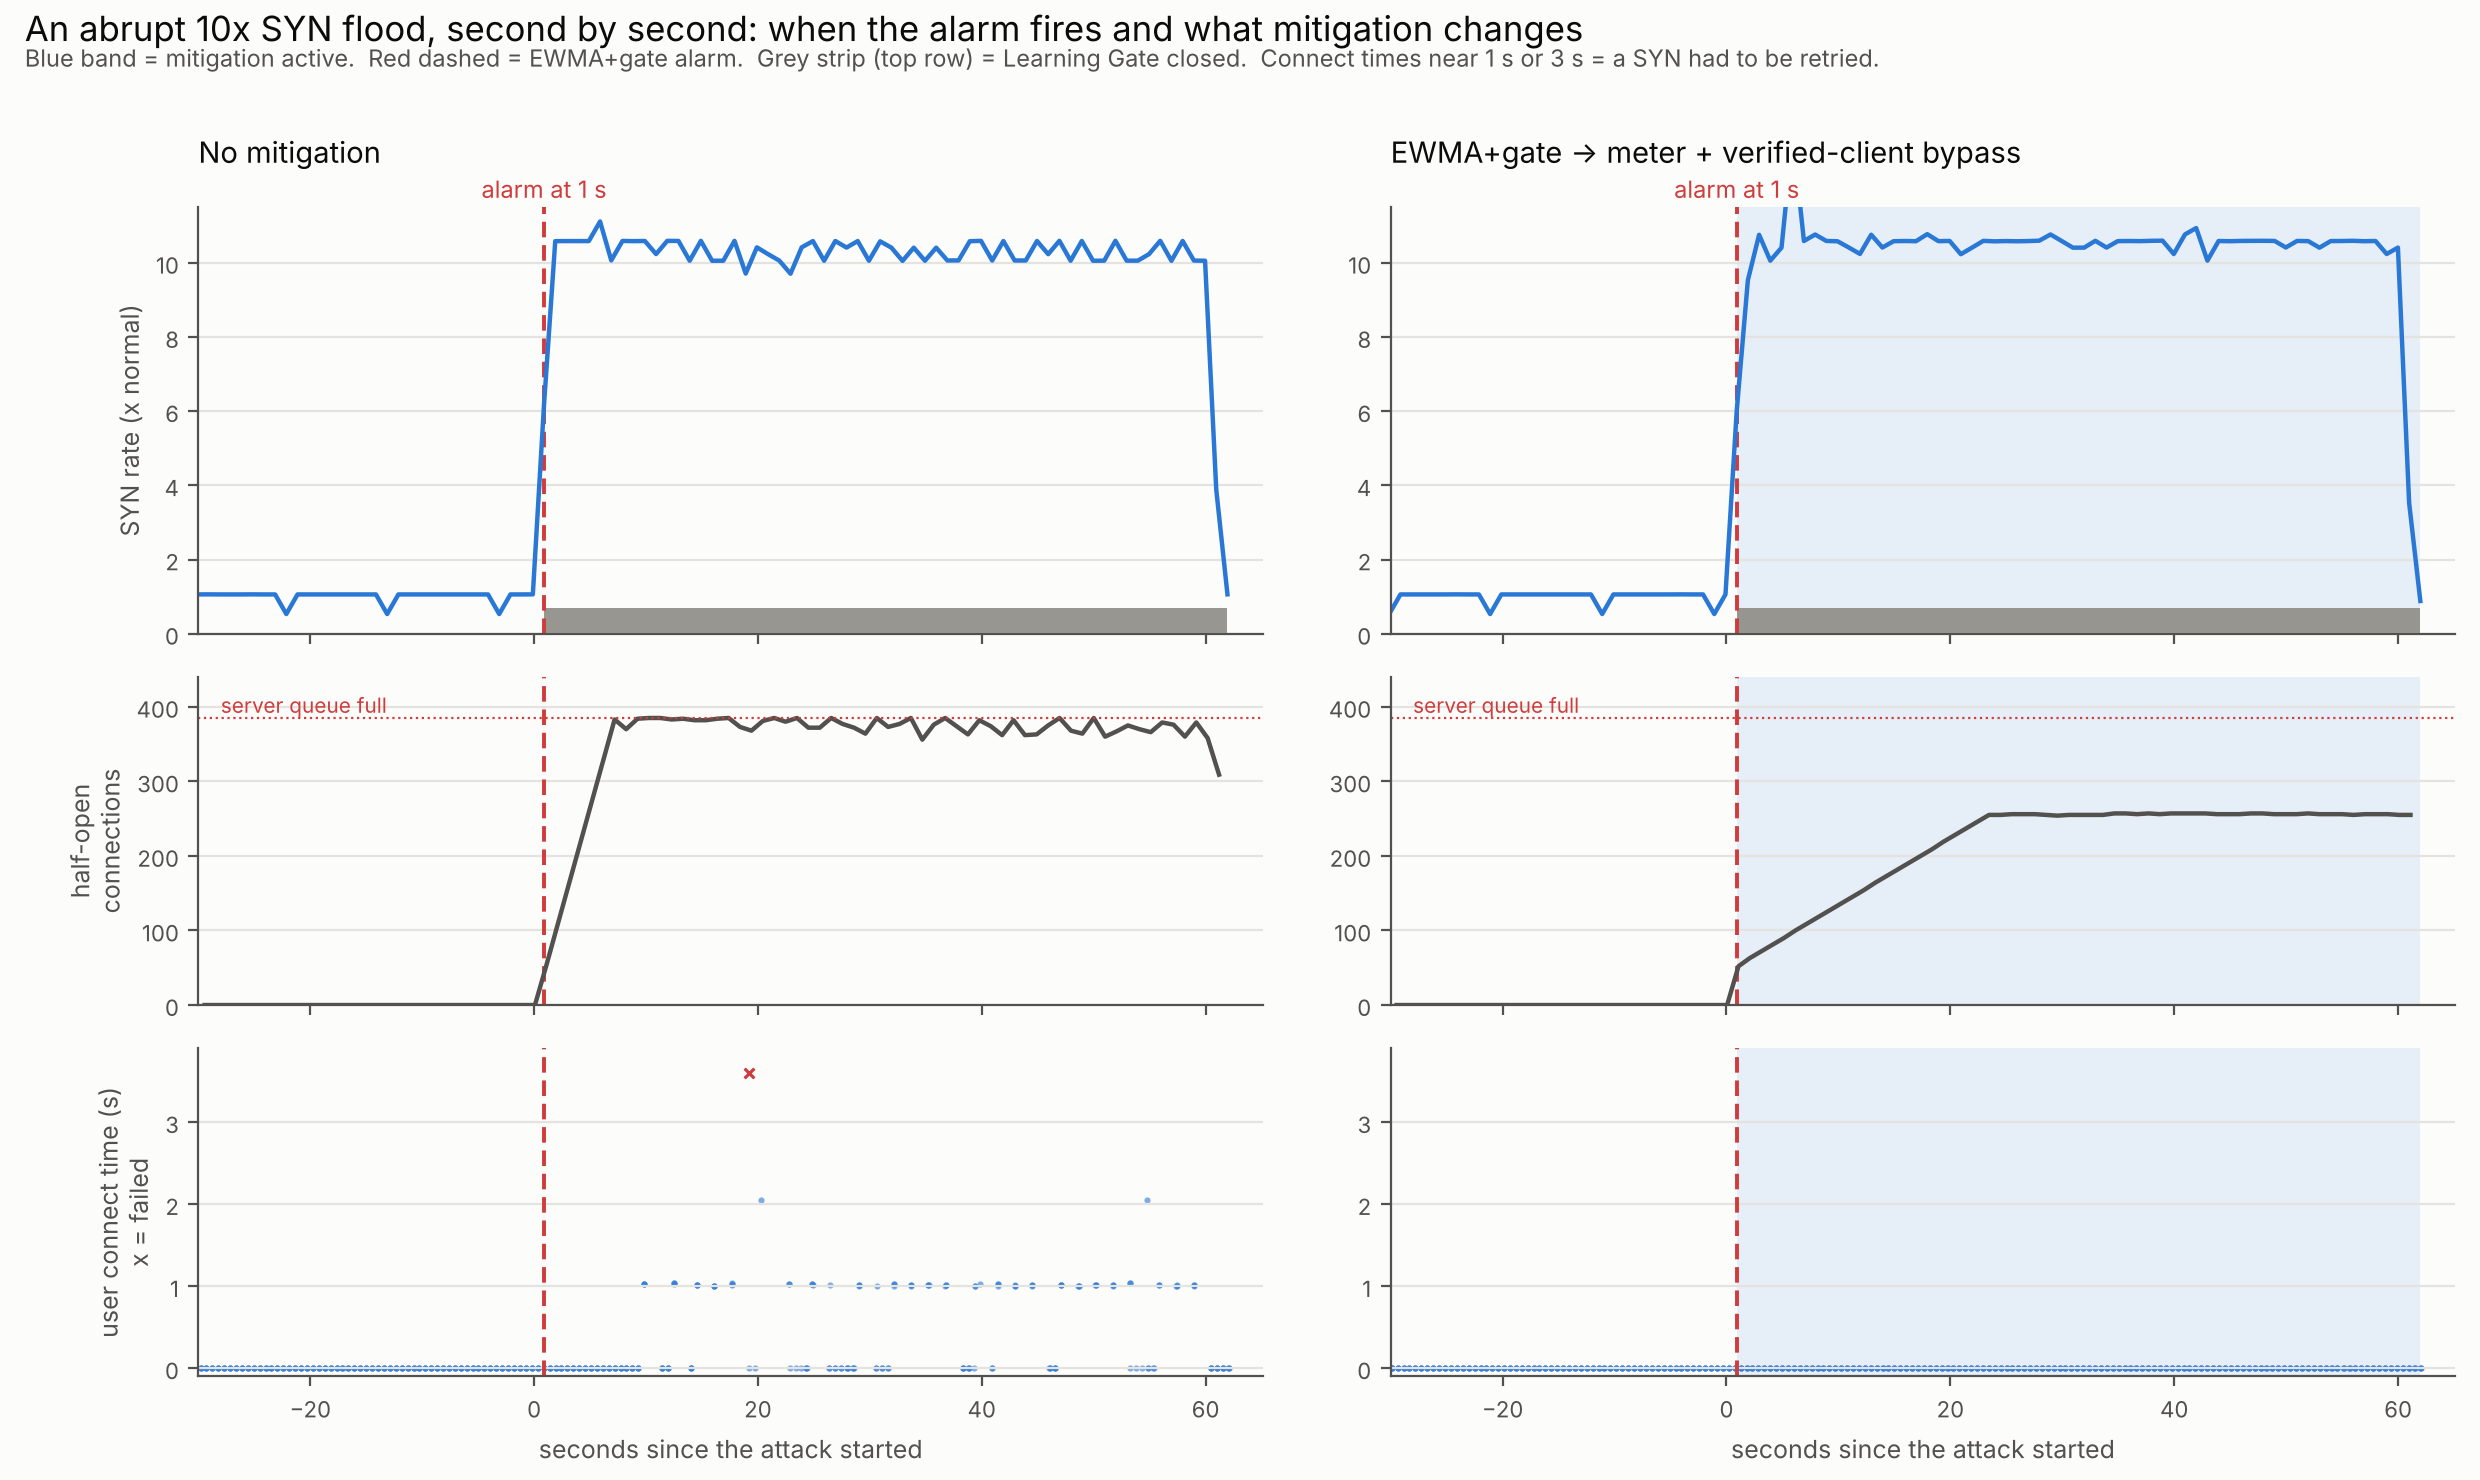
\includegraphics[width=0.85\textwidth]{fig_timeline_abrupt.png}
\caption{An abrupt $10\times$ flood second by second, without mitigation and with meter + verified-client bypass: SYN rate, server half-open connections, and users' connect times.}
\label{fig:timeline}
\end{figure*}

\subsection{Attackers that complete connections}
Bots that use real addresses and complete HTTP requests keep $e_n$ high, so the gate stays open and EWMA+gate learned them (0/3). Static and HST did alarm, but they also alarm on every flash crowd. A drift budget of $\delta \le 2\%$/s detected these bots in all runs (at $4.50\times$ for $\delta = 2\%$/s and $2.25\times$ for $0.5\%$/s), but then false-alarmed on every flash crowd (5/5), as Table~\ref{tab:drift} shows. A rate limit on learning cannot separate a completing attacker from a legitimate crowd that grows at the same speed; we therefore leave the drift budget off by default.

\begin{table}[t]
\centering
\caption{Drift budget $\delta$ with EWMA+gate (offline replay)}
\label{tab:drift}
\setlength{\tabcolsep}{4pt}
\begin{tabular}{lccc}
\toprule
$\delta$ & Spoofed ramp & Completing bots & Crowd FA \\
\midrule
off & 5/5 & 0/3 & 1/5 \\
5\%/s & 5/5 & 0/3 & 1/5 \\
2\%/s & 5/5 & 3/3 & 5/5 \\
0.5\%/s & 5/5 & 3/3 & 5/5 \\
\bottomrule
\end{tabular}
\end{table}

\subsection{Overhead}
EGL adds a constant number of control messages: two statistics requests per second to the server's switch (flow and port statistics), plus one FIN copy per completed connection when verified-client mitigation is enabled. Telemetry uses no Packet-In messages, and the gate's computation is constant per window. \TODO{Measure controller CPU and OpenFlow messages per second with and without EGL, under attack.}

% =====================================================================
\section{Discussion and Limitations}\label{sec:discussion}
% =====================================================================
\textbf{Completing attackers.} EGL defends against attackers who cannot complete connections, which includes all spoofed floods. Application-layer floods from real hosts pass the gate; they need complementary, application-level defences. Combining EGL with per-source evidence (e.g., verified-client counts) is future work.

\textbf{Evidence channel.} The FIN evidence assumes a TCP service that closes connections within the window $W$. Persistent HTTP connections delay FINs; counting RSTs or server ACK bytes are possible alternatives. UDP or QUIC services would need a request--response analogue.

\textbf{Gate versus alarm rule.} EGL repairs what a detector learns, not how it decides. A detector whose alarm rule reacts to any rapid growth (HST here) still false-alarms on flash crowds.

\textbf{Mitigation.} Clients that have never completed a connection must pass the meter during an attack before they are verified. Address-spoofing attackers cannot obtain verification, but an attacker controlling real hosts can.

\textbf{Experimental scope.} The testbed is small, with one controller and one server, and Mininet time is compressed. The attack analysis depends only on the dimensionless quantities $r$, $\beta$ and $\tau$, so the dynamics carry over to slower, real-world ramps. The early-attack and distributed experiments used the user-space datapath and fewer repeats. \TODO{Repeat them on the kernel datapath; evaluate a larger topology, multiple servers and longer, diurnal traffic; compare with the entropy-based detector of \cite{zhang2026time}.}

% =====================================================================
\section{Conclusion}
% =====================================================================
Adaptive DDoS detectors in SDN avoid false alarms on legitimate growth, but by learning from their own verdicts they can be boiled by a slowly increasing attack. We showed this for an EWMA detector and an online machine learning detector, and characterized when such a ramp sustains itself. Evidence-Gated Learning lets a detector learn only while the protected server completes connections, using unforgeable evidence from switch counters. It restored detection of every slow ramp at the analytically predicted point, left legitimate flash crowds undisturbed, and, through verified-client bypass, kept legitimate users served during a flood where a plain rate limit failed them. Attackers that complete real connections remain the main open problem.

\section*{Artifact availability}
Code, raw measurements and the scripts that produce every table and figure are available at \url{https://github.com/Anirudh-N-15/mininet} (branch \texttt{egl}).

\bibliographystyle{IEEEtran}
\bibliography{references}

\end{document}
